\documentclass[a4paper,oneside,12pt]{ctexart}
\usepackage{enumerate,geometry,graphicx,float,setspace,bm,mathrsfs,xcolor,varwidth,framed,amsfonts,amssymb,indentfirst,fancyhdr,BOONDOX-cal,frame}
\usepackage[colorlinks,linkcolor=red,anchorcolor=blue,citecolor=blue,urlcolor=blue]{hyperref}
\usepackage[thmmarks,hyperref]{ntheorem}
\usepackage{amsmath}
\usepackage{listings}
\usepackage{tikz}
\usepackage{asymptote}
\usepackage{cleveref}

\setlength{\headheight}{15pt}
\allowdisplaybreaks[4]
\onehalfspacing
\geometry{centering,left=2.54cm,right=2.54cm,top=3.18cm,bottom=3.18cm}
\pagestyle{fancy}
\fancyhead[L]{\kaishu 强基数学001}
\fancyhead[C]{\kaishu 张卓立}
\fancyhead[R]{\kaishu 2204110786}
\newfontfamily\consolas{Consolas}
\definecolor{matlabgreen}{rgb}{0,0.5,0}
\definecolor{matlabpurple}{rgb}{0.75,0,0.75}
\lstset{
    language=C,
    basicstyle=\consolas,
    keywordstyle=\color{blue},
    commentstyle=\color{matlabgreen}\itshape,
    stringstyle=\color{matlabpurple}\ttfamily,
    frame=single,
    numbers=left,
    numberstyle=\tiny\consolas
}
\tikzset{every picture/.style={line width=0.75pt}} %set default line width to 0.75pt   

\crefname{exercise}{习题}{习题}
\crefname{figure}{图}{图}
\crefname{table}{表}{表}
\crefname{equation}{式}{式}
\crefdefaultlabelformat{(#2#1#3)}

{
    \theoremstyle{plain}
    \theoremheaderfont{\normalfont\bfseries}
    \theorembodyfont{\kaishu}
    \theoremseparator{.}
    \newtheorem{exercise}{习题}
}

{
    \theoremstyle{nonumberplain}
    \theoremheaderfont{\bfseries}
    \theorembodyfont{\normalfont}
    \newtheorem{solution}{解.}
}

{
    \theoremstyle{nonumberplain}
    \theoremheaderfont{\bfseries}
    \theorembodyfont{\normalfont}
    \theoremsymbol{\ensuremath{\blacksquare}}
    \newtheorem{proof}{证明.}
}

\renewcommand{\phi}{\varphi}
\renewcommand{\epsilon}{\varepsilon}
\renewcommand{\emptyset}{\varnothing}
\newcommand{\abs}[1]{\left\vert#1\right\vert}
\newcommand{\norm}[1]{\left\Vert#1\right\Vert}
\renewcommand{\liminf}{\varliminf}
\renewcommand{\limsup}{\varlimsup}

\begin{document}
    \begin{center}
        \bfseries\LARGE
        算法设计与分析作业
    \end{center}

    \begin{exercise}
        \label{ex:4.3}
        若在0-1背包问题中, 各物品依重量递增排列时, 其价值恰好依递减序排列. 对这个特殊的0-1背包问题, 设计一个有效的算法找出最优解, 并说明算法的
        正确性.
    \end{exercise}

    \begin{solution}
        设所给的输入为$W>0,w_i>0,v_i>0,1\leqslant i\leqslant n$. 不妨设$0<w_1\leqslant w_2\leqslant \cdots\leqslant w_n$, 那么$v_1\geqslant v_2\geqslant \cdots\geqslant v_n>0$. 
        则$\frac{v_i}{w_i}\geqslant \frac{v_{i+1}}{w_{i+1}},1\leqslant i\leqslant n-1$. 且当$w_1>W$时问题无解, $w_1\leqslant W$时, 存在0-1背包问题
        的一个最优解, 且$1\notin S$. 对$\forall i\in S$, 取$S_i=S\cup\{1\}-\{i\}$即为满足贪心性质的最优解.
    \end{solution}

    \begin{exercise}
        \label{ex:4.12}
        试设计一个构造图$G$生成树的算法, 使得构造出的生成树的边的最大权值达到最小.
    \end{exercise}

    \begin{solution}
        首先证明最小生成树使得边的最大权值达到最小. 设$G$是一棵最小生成树, $T'$是$G$的一颗使最大权值达到最小的生成树. $e$是$T$中的最大权边, $e'$是$T'$中的最大权边, 
        且$w(e')<w(e)$. 将$e$从$T$中删去后, $T$将分为两个连通分支. 则存在$T'$中的边$e''$连接这两个分支. 将$e''$加入$T$的这两个连通分支得到一棵新的
        生成树$T''=T-e+e''$, $e'$是$T'$的最大权边, 故$w(e'')\leqslant w(e')<w(e)$, 那么$w(T'')=w(T)-w(e)+w(e'')<w(T)$, 与$T$是最小生成树矛盾. 

        综上, 可用Kruscal算法构造$G$的最大权值达到最小的生成树.
    \end{solution}

    \begin{exercise}
        \label{ex:4.13}
        试举例说明如果允许带权有向图中某些边的权为负实数, 则Dijkstra算法不能正确求得从源到其他所有顶点的最短路径长度.
    \end{exercise}

    \begin{solution}
        对于如\cref{fig:负边权有向图}的有向图$G$, 用Dijkstra算法找到顶点1到顶点3的最短路径是1,3, 其长度是1, 但是最短路径是1,2,3, 长度是0.
        \begin{figure}[H]
            \centering
            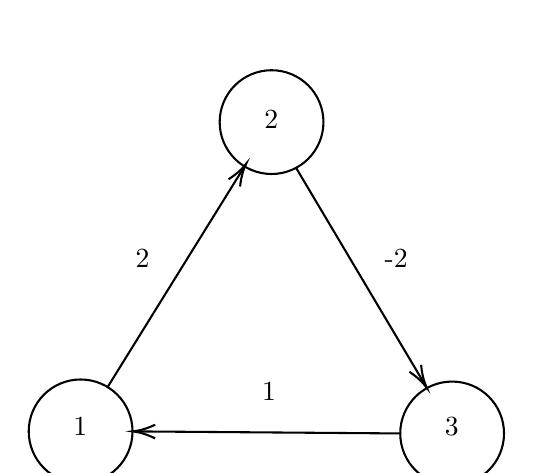
\begin{tikzpicture}[>=latex,x=0.75pt,y=0.75pt,yscale=-1,xscale=1]
                %uncomment if require: \path (0,300); %set diagram left start at 0, and has height of 300
        
                %Shape: Circle [id:dp5674390621255017] 
                \draw   (309,44) .. controls (309,30.19) and (320.19,19) .. (334,19) .. controls (347.81,19) and (359,30.19) .. (359,44) .. controls (359,57.81) and (347.81,69) .. (334,69) .. controls (320.19,69) and (309,57.81) .. (309,44) -- cycle ;
                %Shape: Circle [id:dp2591663517471079] 
                \draw   (217,193) .. controls (217,179.19) and (228.19,168) .. (242,168) .. controls (255.81,168) and (267,179.19) .. (267,193) .. controls (267,206.81) and (255.81,218) .. (242,218) .. controls (228.19,218) and (217,206.81) .. (217,193) -- cycle ;
                %Shape: Circle [id:dp30175075218788283] 
                \draw   (396,194) .. controls (396,180.19) and (407.19,169) .. (421,169) .. controls (434.81,169) and (446,180.19) .. (446,194) .. controls (446,207.81) and (434.81,219) .. (421,219) .. controls (407.19,219) and (396,207.81) .. (396,194) -- cycle ;
                %Straight Lines [id:da4694209047153999] 
                \draw    (254.8,172) -- (320.75,65.7) ;
                \draw [shift={(321.8,64)}, rotate = 121.81] [color={rgb, 255:red, 0; green, 0; blue, 0 }  ][line width=0.75]    (10.93,-3.29) .. controls (6.95,-1.4) and (3.31,-0.3) .. (0,0) .. controls (3.31,0.3) and (6.95,1.4) .. (10.93,3.29)   ;
                %Straight Lines [id:da3605084175531923] 
                \draw    (345.8,66) -- (407.78,170.28) ;
                \draw [shift={(408.8,172)}, rotate = 239.28] [color={rgb, 255:red, 0; green, 0; blue, 0 }  ][line width=0.75]    (10.93,-3.29) .. controls (6.95,-1.4) and (3.31,-0.3) .. (0,0) .. controls (3.31,0.3) and (6.95,1.4) .. (10.93,3.29)   ;
                %Straight Lines [id:da9565501593884216] 
                \draw    (396,194) -- (269,193.02) ;
                \draw [shift={(267,193)}, rotate = 0.44] [color={rgb, 255:red, 0; green, 0; blue, 0 }  ][line width=0.75]    (10.93,-3.29) .. controls (6.95,-1.4) and (3.31,-0.3) .. (0,0) .. controls (3.31,0.3) and (6.95,1.4) .. (10.93,3.29)   ;
        
                % Text Node
                \draw (329,37) node [anchor=north west][inner sep=0.75pt]   [align=left] {2};
                % Text Node
                \draw (237,185) node [anchor=north west][inner sep=0.75pt]   [align=left] {1};
                % Text Node
                \draw (416,185) node [anchor=north west][inner sep=0.75pt]   [align=left] {3};
                % Text Node
                \draw (267,104) node [anchor=north west][inner sep=0.75pt]   [align=left] {2};
                % Text Node
                \draw (387,104) node [anchor=north west][inner sep=0.75pt]   [align=left] {\mbox{-}2};
                % Text Node
                \draw (328,168) node [anchor=north west][inner sep=0.75pt]   [align=left] {1};
        
        
                \end{tikzpicture}
                \caption{负边权有向图}
                \label{fig:负边权有向图}
        \end{figure}
    \end{solution}
\end{document}